%% Elsevier elsarticle draft for Biomedical Signal Processing and Control.
%% The author and affiliation fields below are intentionally left as placeholders.
\documentclass[preprint,12pt]{elsarticle}

\usepackage{amssymb}
\usepackage{amsmath}
\usepackage{booktabs}
\usepackage{graphicx}
\usepackage{url}
\usepackage{array}
\usepackage{multirow}
\usepackage{etoolbox}
\usepackage[section]{placeins}
\usepackage[hidelinks]{hyperref}
\usepackage[expansion=false]{microtype}
% Let lines with long hyphenated compounds stretch instead of overflowing.
\setlength{\emergencystretch}{2em}

% Keep floats in the section that cites them instead of drifting to the end.
\renewcommand{\topfraction}{0.9}
\renewcommand{\bottomfraction}{0.8}
\renewcommand{\textfraction}{0.07}
\renewcommand{\floatpagefraction}{0.75}
\setcounter{topnumber}{3}
\setcounter{totalnumber}{4}

% Table captions sit above the table: separate them from the top rule and
% give rows a little more vertical room.
\AtBeginEnvironment{table}{\setlength{\belowcaptionskip}{6pt}\renewcommand{\arraystretch}{1.15}}
\newcommand{\colhead}[1]{\begin{tabular}[b]{@{}c@{}}#1\end{tabular}}
\AtBeginEnvironment{table*}{\setlength{\belowcaptionskip}{6pt}\renewcommand{\arraystretch}{1.15}}

\journal{Biomedical Signal Processing and Control}

\begin{document}

\begin{frontmatter}

\title{Domain-Adaptive Selective State-Space Learning for Cross-Subject Motor-Imagery EEG Decoding}

\author[aff1]{Author Name\corref{cor1}}
\ead{author@email.com}
\cortext[cor1]{Corresponding author.}

\affiliation[aff1]{organization={Department and Institution},
                   addressline={Street address},
                   city={City},
                   postcode={Postcode},
                   country={Country}}

\begin{abstract}
Cross-subject motor-imagery electroencephalography (MI-EEG) decoding is limited by low signal-to-noise ratios, scarce labeled data, and strong distribution shifts across subjects and sessions. We propose a domain-adaptive selective state-space framework for this setting. A multi-kernel temporal convolutional front-end with depthwise spatial filtering and channel-group attention extracts local spectral--spatial features. Five selective state-space blocks with alternating forward and backward scans then model long-range temporal context at a cost linear in sequence length, and a convolutional shortcut with a grouped dilated temporal convolutional network fuses local and global information. To reduce cross-subject shift, the framework combines per-subject Riemannian alignment, gradient-reversal adversarial learning, and multi-kernel maximum mean discrepancy at the temporal and trial levels. At inference time, an information-maximization stage adapts only normalization parameters using unlabeled evaluation-session trials; their labels remain hidden until scoring. On BCI IV-2a, Ours achieved $75.81\pm10.63\%$ session-2 accuracy and a Cohen's $\kappa$ score of $67.70\pm14.20$ on the $\times100$ scale across nine LOSO target subjects. Code will be released at \url{https://github.com/USERNAME/REPOSITORY}.
\end{abstract}

\begin{keyword}
motor imagery \sep electroencephalography \sep brain--computer interface \sep selective state-space model \sep Mamba \sep domain adaptation \sep test-time adaptation
\end{keyword}

\end{frontmatter}

\section{Introduction}
\label{sec:introduction}

Motor-imagery brain--computer interfaces (MI-BCIs) translate internally generated movement intentions into commands without requiring overt muscular activity. Their non-invasive electroencephalography (EEG) interface and millisecond temporal resolution make them attractive for neurorehabilitation, assistive communication, and human--machine control. Reliable decoding nevertheless remains difficult. MI-related sensorimotor rhythms, observed as event-related desynchronization and synchronization (ERD/ERS) \cite{pfurtscheller1999erd}, are weak, noisy, non-stationary, and distributed over both time and scalp location. More importantly for practical deployment, their statistical distributions vary markedly among subjects and between recording sessions. A model trained for one user can therefore lose accuracy on a new user, while collecting and labeling a separate calibration set for every user is slow and burdensome. Cross-subject decoding consequently requires two capabilities at once: learning discriminative spatial--temporal structure from limited EEG trials and remaining robust to a previously unseen subject distribution.

Early MI decoders addressed the first requirement through signal processing and shallow machine learning. Common spatial pattern (CSP) learns spatial filters that maximize the variance contrast between two classes and remains one of the most influential MI feature extractors \cite{ramoser2000optimal}. Its success also exposes its limitations: the learned projection is sensitive to the available training trials, conventional CSP is naturally binary, and performance depends strongly on the selected frequency interval. Filter-bank CSP (FBCSP) improved this pipeline by applying CSP to multiple sub-bands and selecting discriminative band-specific features \cite{ang2012filterbank}. Although effective and interpretable, CSP-family pipelines separate filtering, feature selection, and classification into manually designed stages. They do not learn task-dependent temporal, spectral, and spatial representations jointly, and their subject-specific covariance structure transfers poorly when the user changes.

End-to-end convolutional neural networks (CNNs) reduced this dependence on handcrafted features. Deep and shallow ConvNets demonstrated that temporal and spatial EEG filters can be learned directly from minimally processed signals \cite{schirrmeister2017deep}. EEGNet subsequently used depthwise and separable convolutions to encode frequency-specific spatial filters with a small parameter budget \cite{lawhern2018eegnet}. These designs provide useful inductive biases for EEG: short temporal kernels capture local oscillatory patterns, depthwise spatial kernels combine electrodes, and pooling suppresses small temporal translations. Multi-scale or filter-bank convolution further reflects the fact that MI information is not confined to a single temporal scale. However, a CNN represents distant time points only after stacking layers, enlarging kernels, or using dilation. Its local bias alone may therefore be insufficient to model the full evolution of event-related desynchronization and synchronization within a trial.

Recent work has coupled convolution with attention or temporal sequence modules to capture local and global information jointly. EEG Conformer places self-attention after a convolutional tokenizer so that local temporal--spatial features can interact globally \cite{song2023eegconformer}. ATCNet combines attention, sliding temporal windows, and a temporal convolutional network (TCN), with dilated convolutions refining the time course of MI features \cite{altaheri2023atcnet}. More recently, TCFormer integrated a multi-kernel CNN, grouped-query Transformer layers, and a grouped TCN head \cite{altaheri2025tcformer}. This progression establishes a useful architectural principle: EEG-specific convolution should preserve local spectral and spatial structure, whereas a sequence encoder should capture global context. Yet self-attention explicitly constructs pairwise token interactions, giving quadratic time and memory complexity in sequence length \cite{vaswani2017attention}. This can be unnecessarily expensive for high-resolution or long-window EEG, and its flexible global operator can be data-hungry in the small-sample regimes typical of BCI experiments.

Architecture alone does not resolve inter-subject distribution shift. Domain generalization (DG) learns invariant representations from multiple labeled source subjects and deploys one model on an unseen target without accessing its data. Recent MI studies have explored spatial--temporal Transformers with DG \cite{liu2023stdg}, multi-source marginal and conditional alignment \cite{zhong2025eegdg}, and invariant spectral representations with correlation alignment \cite{zheng2025crosssubject}. DG is appealing for strict plug-and-play operation, but it cannot use the actual target distribution and may miss subject-specific shifts that were not represented by the sources. Domain adaptation (DA), in contrast, exploits unlabeled target trials while preserving a label-free target protocol. These settings must not be conflated: a method that observes unlabeled target EEG during training or adaptation is unsupervised DA rather than zero-shot DG.

EEG domain adaptation has developed along complementary geometric, discrepancy-based, and adversarial directions. Riemannian transfer learning and Euclidean alignment reduce covariance mismatch before classification by re-centering or whitening trials in a common space \cite{zanini2018riemannian,he2020euclidean}. At the representation level, deep adaptation networks minimize a multi-kernel maximum mean discrepancy (MK-MMD) between source and target features \cite{long2015dan}. Domain-adversarial neural networks instead train a feature extractor to confuse a domain discriminator through gradient reversal \cite{ganin2016dann}; conditional adversarial variants use class predictions to preserve discriminative structure during alignment and have also been applied to MI-EEG \cite{tang2020cdan}. For cross-subject MI decoding, HADANet combines a hierarchical convolutional extractor and hybrid attention with joint adversarial and MK-MMD alignment \cite{wu2026hadanet}, and prototype-based adaptation networks additionally exploit local class information in the target domain \cite{zhang2024prototypeda}. These approaches are valuable but not risk-free. Global marginal alignment can mix class modes, and forcing a poorly matched or low-confidence target toward the sources can cause negative transfer. Moreover, aligning only the final trial vector may overlook a mismatch in the temporal representation from which that vector was produced.

Test-time adaptation offers another opportunity after source training. Information-maximization methods encourage confident yet globally diverse target predictions without requiring labels \cite{liang2020shot}, while TENT showed that adapting only normalization statistics and affine parameters through entropy minimization can be an efficient response to distribution shift \cite{wang2021tent}. For EEG, unrestricted target fine-tuning would be hazardous because target datasets are small and model predictions can initially be unreliable. A constrained update space and a diversity term are therefore important safeguards against overfitting and single-class collapse.

Structured state-space models such as S4 provide a promising alternative to attention for modeling long sequences efficiently \cite{gu2022s4}. Building on this family, Mamba makes state-transition quantities input-dependent, enabling a recurrent state to selectively retain or discard information while maintaining linear scaling with sequence length \cite{gu2024mamba}. Such selective memory is well matched to EEG, where discriminative activity is sparse, temporally structured, and embedded in noise. Recent MI-EEG decoders have accordingly combined convolutional feature extractors with Mamba blocks \cite{guo2025mimamba,yang2025stmamba}. These studies focus primarily on decoder architecture, leaving open how a selective state-space encoder should be combined with unlabeled target adaptation under a leakage-controlled cross-subject protocol. Moreover, replacing an EEG decoder with a generic state-space stack would discard useful domain knowledge. A pure unidirectional recurrence also introduces a directional bias even though an offline MI trial is available in full, and a sequence module should not be expected to replace explicit electrode filtering or local temporal extraction.

Motivated by these observations, this paper proposes a hybrid, target-aware framework for cross-subject MI-EEG decoding. The model first applies three parallel temporal convolutions to the same EEG trial to capture complementary temporal scales. Their features are concatenated and processed by depthwise spatial convolution, which learns multiple electrode projections for each temporal feature. Grouped pointwise and temporal convolutions retain scale structure, and channel-group attention recalibrates the resulting branches. This convolutional representation is tokenized and passed through five lightweight selective state-space blocks. Their scan directions alternate forward and backward, allowing successive layers to incorporate both temporal directions without duplicating a bidirectional block at every depth. A direct convolutional shortcut is concatenated with the state-space output so that global contextualization does not erase local EEG evidence. Finally, a grouped TCN with increasing dilation refines multi-scale temporal dynamics before classification.

The proposed framework couples this encoder with hierarchical unsupervised domain adaptation that extends the hybrid adversarial--MK-MMD alignment of HADANet \cite{wu2026hadanet}. First, per-subject covariance alignment is fitted only on the earlier target-adaptation data. During training, labeled source trials and unlabeled target-adaptation trials share the same feature extractor. A gradient-reversal discriminator promotes domain confusion, MK-MMD aligns pooled trial representations, and a lighter temporal MK-MMD aligns the time-averaged TCN feature sequences before trial aggregation. At inference time, information maximization updates only BatchNorm affine parameters using the unlabeled EEG from the evaluation session itself. Evaluation labels remain hidden throughout training, adaptation, preprocessing-statistic estimation, and checkpoint selection and are used only to compute final metrics.

The main contributions of this work are summarized as follows:
\begin{itemize}
    \item We develop an EEG-specific encoder that combines multi-kernel temporal filtering, depthwise electrode filtering, a local convolutional shortcut, five alternating-direction selective state-space blocks, and a grouped dilated TCN. The design preserves local spatial--spectral priors while modeling long-range temporal context without pairwise self-attention.
    \item We introduce hierarchical cross-subject alignment that combines leakage-safe covariance normalization, adversarial domain confusion, final-representation MK-MMD, and temporal MK-MMD.
    \item We incorporate a constrained source-free information-maximization stage in which only normalization affine parameters are adapted from unlabeled target trials, while a diversity objective discourages prediction collapse.
    \item We formulate a reproducible leave-one-subject-out evaluation protocol that keeps target labels out of training, adaptation, checkpoint selection, and preprocessing-statistic estimation, thereby separating the proposed UDA setting clearly from both supervised target calibration and target-free DG.
\end{itemize}

The remainder of this paper describes the datasets, model and adaptation objectives, leakage-controlled experimental protocol, planned result reporting, ablation design, discussion, and conclusions.

\section{Datasets}
\label{sec:datasets}

Three public MI-EEG datasets are used to examine whether the same decoder transfers across different numbers of electrodes, classes, subjects, and recording sessions. Dataset access and event extraction are implemented through the MOABB/Braindecode interface; this choice provides a common representation of subjects, sessions, runs, and event windows and supports reproducible benchmarking \cite{jayaram2018moabb}. Table~\ref{tab:datasets} summarizes the properties relevant to the present work.

\begin{table*}[!htbp]
\centering
\caption{Summary of the MI-EEG datasets (EOG channels excluded).}
\label{tab:datasets}
\small
\setlength{\tabcolsep}{4.5pt}
\begin{tabular}{lcccl}
\toprule
Dataset & Subjects & Channels & Sessions & Classes \\
\midrule
BCI IV-2a & 9 & 22 & 2 & left hand, right hand, feet, tongue \\
BCI IV-2b & 9 & 3  & 5 & left hand, right hand \\
Zhou2016  & 4 & 14 & 3 & left hand, right hand, feet \\
\bottomrule
\end{tabular}
\end{table*}

\subsection{BCI Competition IV-2a}
\label{subsec:bcic2a}

BCI Competition IV dataset 2a contains recordings from nine participants. Each participant completed two sessions on different days, and each session contains 288 trials distributed equally over imagined left-hand, right-hand, both-feet, and tongue movements. Signals were acquired from 22 EEG electrodes and three EOG electrodes at 250~Hz; only the EEG electrodes are supplied to the classifier. The original recordings were hardware band-pass filtered between 0.5 and 100~Hz and notch filtered at 50~Hz \cite{tangermann2012review}. The implementation uses the event-defined MI interval exposed by MOABB, rescales volts to microvolts, and does not apply an additional frequency filter. The first recording session is denoted session~1 and the second is denoted session~2 throughout this paper.

\subsection{BCI Competition IV-2b}
\label{subsec:bcic2b}

BCI Competition IV dataset 2b contains two-class left- versus right-hand MI recordings from nine participants. Three bipolar EEG derivations centered on C3, Cz, and C4 were sampled at 250~Hz, together with three EOG channels that are excluded from decoding. Each participant completed five sessions: the first three form the calibration portion and the final two form the original evaluation portion \cite{tangermann2012review}. The present loader follows this natural chronological separation. The event-defined MI window is used after removing the final 0.5~s through the configured stop offset. This dataset tests whether the method remains useful when spatial coverage is reduced from 22 electrodes to only three.

\subsection{Zhou2016}
\label{subsec:zhou2016}

The Zhou2016 dataset contains four participants, each recorded in three sessions separated by days to months. A session consists of two runs of 75 trials, with 25 trials per class, giving 450 trials per participant. The three MI classes are left hand, right hand, and feet. EEG was recorded from 14 electrodes at 250~Hz. Each trial contains a 5-s visual arrow period during which the indicated imagery is performed, followed by a 4-s rest period \cite{zhou2016trialselection}. We therefore extract exactly the first 5.0~s from cue onset rather than including the subsequent rest interval. The public data are loaded through the MOABB representation, whose consistent dataset API is useful for avoiding dataset-specific indexing errors \cite{jayaram2018moabb}.

\section{Proposed Method}
\label{sec:method}

Figure~\ref{fig:architecture_overview} presents the complete learning and inference pipeline. The source and target streams share one encoder, while supervision and adaptation objectives branch only after representation extraction. The figure distinguishes joint UDA training on earlier target sessions, label-free information-maximization adaptation on the evaluation-session EEG at inference time, and subsequent scoring with labels that were withheld from both stages.

\begin{figure*}[!htbp]
    \centering
    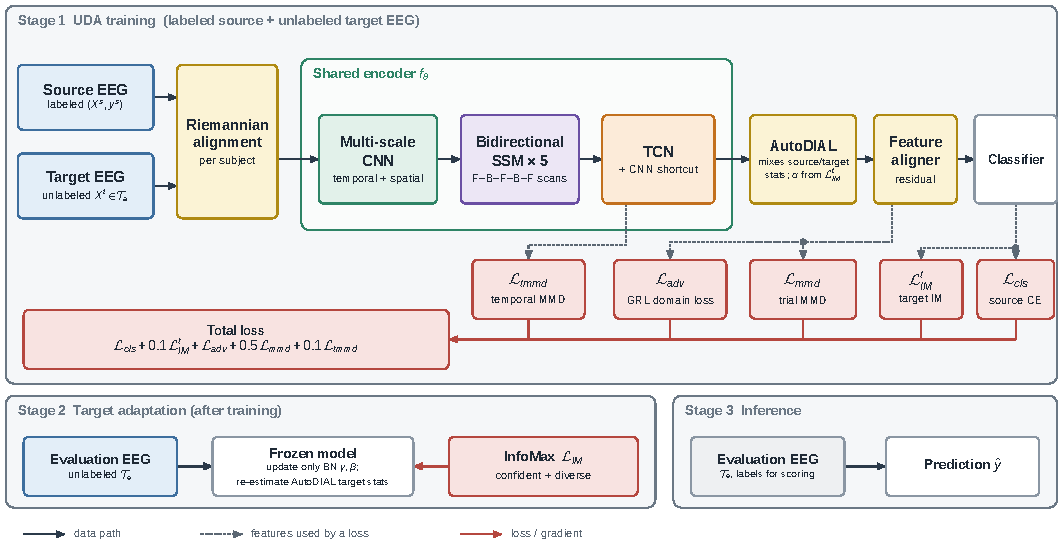
\includegraphics[width=\textwidth]{figures/architecture_overview.pdf}
    \caption{Overview of the proposed framework in one LOSO fold. Stage~1 trains the shared encoder with labeled source EEG and earlier unlabeled target EEG; Stage~2 performs label-free IM-TTA on the evaluation-session EEG; Stage~3 scores the adapted model using labels withheld from all preceding stages.}
    \label{fig:architecture_overview}
\end{figure*}

\subsection{Problem formulation}

Let $\mathcal{S}=\{(X_i^s,y_i^s)\}_{i=1}^{N_s}$ denote labeled trials from all source subjects, $\mathcal{T}_a=\{X_j^a\}_{j=1}^{N_a}$ the earlier unlabeled target sessions used during Stage~1 UDA, and $\mathcal{T}_e=\{X_j^e\}_{j=1}^{N_e}$ the later target sessions used for evaluation. A trial is represented as $X\in\mathbb{R}^{C\times T}$. In each LOSO fold, the model is trained with labeled $\mathcal{S}$ and unlabeled $\mathcal{T}_a$. After checkpoint selection, IM-TTA may use the signal values of $\mathcal{T}_e$ without labels; the evaluation labels are revealed only after adaptation to compute the reported metrics.

\subsection{Leakage-safe signal alignment}
\label{subsec:ra}

The implementation optionally applies a separate Riemannian whitening operator to every subject. For one subject, covariance matrices are estimated from that subject's available adaptation or training trials with Oracle Approximating Shrinkage. Their affine-invariant Riemannian mean is denoted by $\bar{R}$. Every trial belonging to the same subject is transformed as
\begin{equation}
    \widetilde{X}=\bar{R}^{-1/2}X .
\end{equation}
For a source subject, $\bar{R}$ is fitted using only that source subject's training sessions and then applied to its validation sessions. For the target subject, it is fitted only on $\mathcal{T}_a$ and then frozen before application to $\mathcal{T}_e$. This construction follows the motivation of Riemannian transfer and alignment methods \cite{zanini2018riemannian,he2020euclidean}. Evaluation-session signals are used by IM-TTA, but they do not update the covariance-alignment transform or the standardization statistics.

\subsection{Multi-scale temporal and spatial convolution}
\label{subsec:conv_frontend}

The convolutional front-end and its tensor dimensions are detailed in Fig.~\ref{fig:encoder_detail}. Its output $H_c$ feeds both the selective state-space encoder (Section~\ref{subsec:ssm}) and a direct local shortcut; the two paths are reunited before the TCN (Section~\ref{subsec:tcn}).

\begin{figure*}[!htbp]
    \centering
    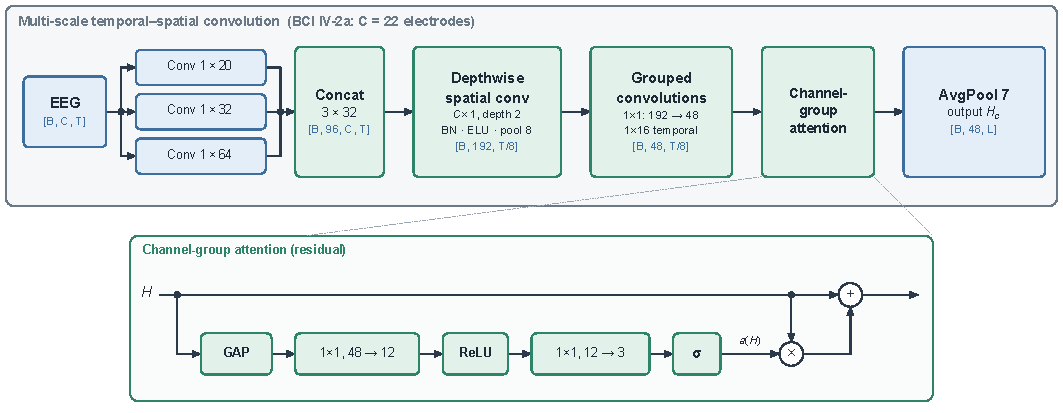
\includegraphics[width=\textwidth]{figures/encoder_detail.pdf}
    \caption{Multi-scale temporal--spatial convolutional front-end, illustrated for BCI IV-2a. Three temporal kernels are followed by depthwise electrode filtering, grouped channel reduction, grouped temporal refinement, and residual channel-group attention, producing the sequence $H_c$.}
    \label{fig:encoder_detail}
\end{figure*}

Following the multi-kernel temporal front-end of TCFormer \cite{altaheri2025tcformer}, the convolutional block first reshapes a mini-batch to $B\times 1\times C\times T$. Three temporal branches then process the same trial using kernels of length 20, 32, and 64 samples:
\begin{equation}
    H_k=\operatorname{BN}\!\left(\operatorname{Conv}_{1\times k}(X)\right),
    \qquad k\in\{20,32,64\}.
\end{equation}
Asymmetric zero padding for even kernels preserves the original time length. Each branch produces 32 maps, and concatenation gives 96 maps while retaining the identity of the three scales.

A depthwise convolution whose spatial kernel spans all $C$ electrodes is applied independently to every temporal map. With a depth multiplier of two, each of the 96 inputs learns two electrode projections, resulting in 192 maps. Batch normalization and ELU activation follow the spatial filter. Average pooling by eight and dropout reduce temporal resolution and regularize the representation. A grouped $1\times 1$ convolution then maps 192 channels to 48 channels, with 16 channels retained for each temporal-scale group. A grouped temporal convolution with kernel length 16 further refines each scale without mixing the groups.

Channel-group attention assigns one data-dependent sigmoid coefficient to each temporal-scale group. Global average pooling is followed by grouped $1\times1$ projections $48\rightarrow12\rightarrow3$, ReLU, and sigmoid. Its output is used residually:
\begin{equation}
    H_{\mathrm{att}}=H+H\odot a(H),
\end{equation}
where the three coefficients in $a(H)$ are broadcast over the 16 channels in their corresponding groups. A second average-pooling layer with factor seven and dropout produces a sequence $H_c\in\mathbb{R}^{B\times48\times L}$.

\subsection{Alternating selective state-space encoder}
\label{subsec:ssm}

Before sequence modeling, a $1\times1$ convolution, batch normalization, and SiLU activation mix the 48 convolutional channels. The sequence is then processed by five lightweight selective state-space blocks in the order forward--backward--forward--backward--forward. A backward block reverses the temporal axis before its recurrence and reverses the output afterward. Consequently, the stack incorporates evidence from both temporal directions while each individual block retains the parameter cost of a single scan. The internal structure of one block is shown in Fig.~\ref{fig:ssm_block}.

\begin{figure*}[!htbp]
    \centering
    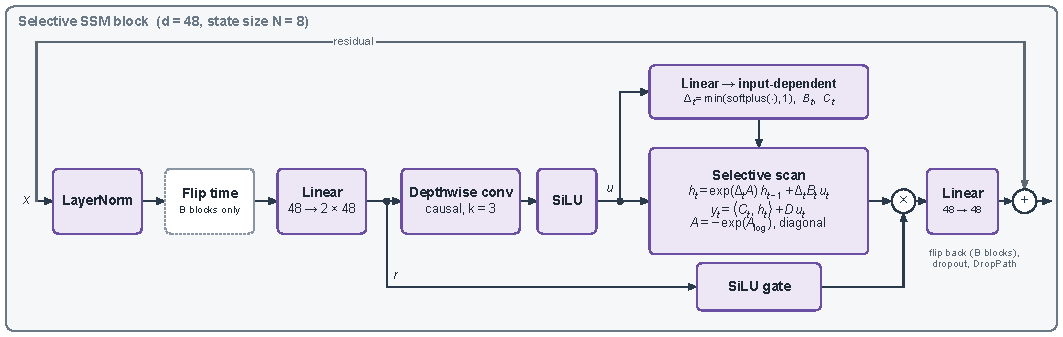
\includegraphics[width=\textwidth]{figures/ssm_block.pdf}
    \caption{Structure of one selective SSM block. Backward (B) blocks reverse the time axis before the mixer and restore it afterwards; forward (F) blocks skip both flips.}
    \label{fig:ssm_block}
\end{figure*}

Each block normalizes its input tokens and projects them into a value stream and a SiLU-gated stream. A causal depthwise temporal convolution of length three followed by SiLU supplies local context to the value stream, giving $u_t$. Following the diagonal state-space formulation used in structured SSMs \cite{gu2022s4}, the input-dependent step size $\Delta_t$ and state projections $B_t$ and $C_t$ parameterize a selective recurrence of the form
\begin{align}
    A &= -\exp(A_{\log}), \\
    h_t &= \exp(\Delta_t A)\odot h_{t-1}
       + \Delta_t B_t\odot u_t, \\
    z_t &= C_t^\top h_t + d_{\mathrm{skip}}\odot u_t .
\end{align}
The block output is projected after modulation by the learned gate and added to the residual stream. The stable negative diagonal $A$ and input-dependent transition quantities implement a lightweight selective-memory mechanism inspired by Mamba \cite{gu2024mamba}. This is a simplified PyTorch implementation rather than the official Mamba block or its hardware-aware parallel selective-scan kernel. The code uses a state dimension of eight, dropout of 0.4, and a depth-dependent stochastic-depth schedule. Unlike pairwise self-attention, the recurrent scan has linear sequence-length scaling.

\subsection{Local--global fusion, TCN, and classification}
\label{subsec:tcn}

The output of the fifth state-space block is reduced from 48 to 16 channels with a pointwise convolution. It is concatenated with the untouched 48-channel convolutional sequence $H_c$, yielding 64 channels. This shortcut protects local temporal--spatial evidence from being overwritten by the global sequence encoder. The fusion, TCN, and classification head are shown in Fig.~\ref{fig:tcn_head}.

\begin{figure*}[!htbp]
    \centering
    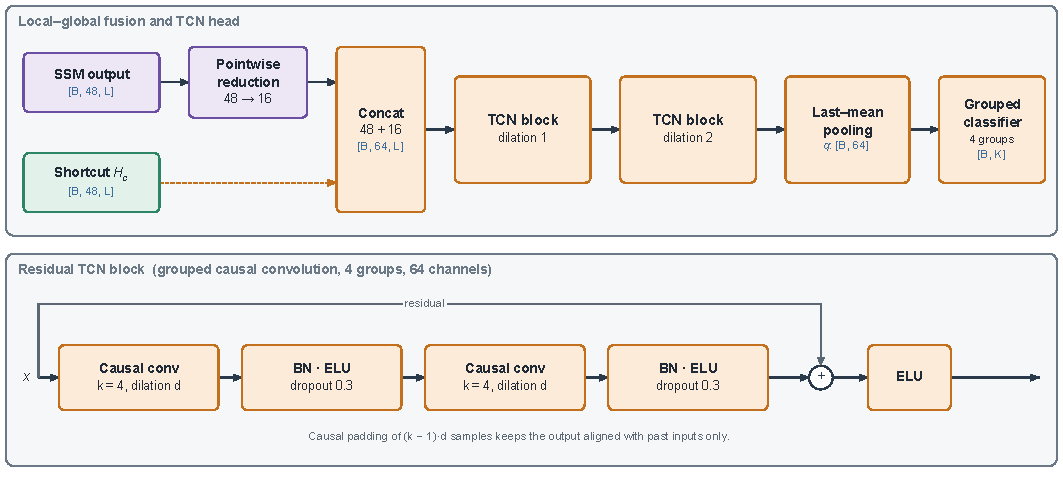
\includegraphics[width=\textwidth]{figures/tcn_head.pdf}
    \caption{Local--global fusion and TCN head. Top: the reduced SSM output is concatenated with the shortcut $H_c$ and refined by two residual TCN blocks before last--mean pooling and grouped classification. Bottom: structure of one residual TCN block.}
    \label{fig:tcn_head}
\end{figure*}

Two residual TCN blocks then refine the fused sequence. Each block contains two causal grouped one-dimensional convolutions with kernel length four, batch normalization, ELU, and dropout. Dilations one and two enlarge the receptive field while preserving temporal order. The final trial representation is
\begin{equation}
    q=\frac{1}{2}\left(H_{\mathrm{TCN}}[:,:,-1]
      +\frac{1}{L}\sum_{t=1}^{L}H_{\mathrm{TCN}}[:,:,t]\right),
\end{equation}
which balances the last causal state with the mean over the whole sequence. A grouped norm-constrained $1\times1$ classifier produces one class-logit contribution per feature group, and learned softmax weights combine the four group contributions.

\subsection{Hierarchical unsupervised domain adaptation}
\label{subsec:uda}

The 64-dimensional pooled representation first passes through a residual feature aligner comprising layer normalization and a $64\rightarrow128\rightarrow64$ GELU multilayer perceptron with dropout 0.3 and a final layer normalization. Its residual scale is initialized to 0.1 so that adaptation begins close to the source-trained representation.

As shown in Fig.~\ref{fig:architecture_overview}, temporal discrepancy is measured before trial aggregation, whereas pooled-feature discrepancy, adversarial domain confusion, and source classification act on the aligned trial vector. Only $\mathcal{L}_{\mathrm{cls}}$ consumes class labels, and the later information-maximization stage updates only normalization affine parameters.

Three complementary losses are then computed. First, source cross-entropy preserves class discrimination:
\begin{equation}
    \mathcal{L}_{\mathrm{cls}}
    =-\frac{1}{N_s}\sum_i \log p_\theta(y_i^s\mid X_i^s).
\end{equation}
Second, a gradient-reversal layer connects pooled source and target features to a binary domain discriminator \cite{ganin2016dann}. The discriminator uses projections $64\rightarrow128\rightarrow64\rightarrow1$, LeakyReLU activations, and dropout 0.3. Its reversal coefficient follows
\begin{equation}
    \alpha(p)=\frac{2}{1+\exp(-10p)}-1,
\end{equation}
where $p$ is normalized training progress. The resulting binary cross-entropy is denoted $\mathcal{L}_{\mathrm{adv}}$.

Third, MK-MMD measures source--target discrepancy using five Gaussian kernels with data-dependent bandwidth \cite{long2015dan}. Features are first normalized to unit $\ell_2$ norm, and the implementation removes within-domain diagonal terms to obtain an unbiased estimate when both mini-batches contain at least two trials. MK-MMD is evaluated on both the aligned trial vectors, giving $\mathcal{L}_{\mathrm{mmd}}$, and the time-averaged TCN feature sequences, giving $\mathcal{L}_{\mathrm{tmmd}}$. The temporal term introduces no additional trainable parameters and discourages alignment that matches only the final pooled vector.

The complete training objective is
\begin{equation}
    \mathcal{L}
    =\mathcal{L}_{\mathrm{cls}}
     +\mathcal{L}_{\mathrm{adv}}
     +0.5\,\mathcal{L}_{\mathrm{mmd}}
     +0.1\,\mathcal{L}_{\mathrm{tmmd}}.
\label{eq:total_loss}
\end{equation}
Only source labels contribute to Eq.~\eqref{eq:total_loss}; the target branch receives EEG samples without labels.

\subsection{Constrained information-maximization adaptation}
\label{subsec:imtta}

After source/UDA training, all model parameters are frozen except the affine weights and biases of BatchNorm layers. At inference time, five passes over the unlabeled evaluation-session set $\mathcal{T}_e$ are performed with Adam at a learning rate of $10^{-4}$. Let $p_j$ denote an evaluation-session prediction and $\bar{p}=N_e^{-1}\sum_j p_j$. The information-maximization objective is
\begin{equation}
    \mathcal{L}_{\mathrm{IM}}
    =\frac{1}{N_e}\sum_j H(p_j)-H(\bar{p}).
\end{equation}
The first term promotes confident predictions, whereas the second encourages a diverse target class marginal and reduces the risk of collapse to one class \cite{liang2020shot,wang2021tent}. This is a transductive, label-free test-time adaptation step: $\mathcal{T}_e$ signals are available to the adaptation objective, but their labels are withheld until adaptation has finished and predictions are scored. No evaluation label or evaluation metric is used to update the model or select a checkpoint.

\section{Experimental Protocol}
\label{sec:experiments}

\subsection{Chronological LOSO protocol with test-time adaptation}
\label{subsec:clean_protocol}

One subject is held out in each LOSO fold. All remaining subjects are sources; the held-out participant is the target. Table~\ref{tab:protocol} specifies the chronological session split. Earlier target sessions are used without labels during Stage~1 UDA. The later evaluation sessions remain unavailable during model training, preprocessing-statistic fitting, and checkpoint selection; at inference time, their EEG signals are passed without labels to IM-TTA, after which the adapted model is scored using the withheld labels. This is the primary protocol for headline comparisons.

\begin{table*}[!htbp]
\centering
\caption{Chronological session allocation in each LOSO fold. Evaluation-session EEG is available without labels only to IM-TTA at inference time; its labels are used afterward solely for scoring.}
\label{tab:protocol}
\small
\setlength{\tabcolsep}{5pt}
\begin{tabular}{lcccc}
\toprule
\multirow{2}{*}{Dataset} & \multicolumn{2}{c}{Source subjects (labeled)} & \multicolumn{2}{c}{Target subject} \\
\cmidrule(lr){2-3}\cmidrule(lr){4-5}
 & Training & Validation & \colhead{Stage~1 UDA\\(unlabeled)} & \colhead{IM-TTA + evaluation\\(labels withheld)} \\
\midrule
BCI IV-2a & session 1      & session 2      & session 1      & session 2 \\
BCI IV-2b & sessions 1--3  & sessions 4--5  & sessions 1--3  & sessions 4--5 \\
Zhou2016  & sessions 1--2  & session 3      & session 1      & sessions 2--3 \\
\bottomrule
\end{tabular}
\end{table*}

For BCI IV-2a, this split yields nine folds; for BCI IV-2b, nine folds; and for Zhou2016, four folds. The target identifier changes between folds, but the split rule and hyperparameters remain fixed. The checkpoint with the highest source-validation accuracy is selected before IM-TTA. Neither evaluation-session labels nor evaluation metrics participate in adaptation or checkpoint selection. Stage~1 adversarial/MK-MMD training uses the earlier unlabeled target-adaptation loader, whereas Stage~2 IM-TTA uses the later unlabeled evaluation loader immediately before predictions are scored.


\subsection{Preprocessing and augmentation}
\label{subsec:preprocessing}

Only EEG channels are retained. Signals are resampled to 250~Hz and converted from volts to microvolts. No additional digital band-pass filter is applied in the model configuration, because the public BCI Competition recordings already include acquisition filtering and the network learns its temporal filters from the signal. BCI IV-2a uses the complete MOABB event window; BCI IV-2b removes 0.5~s from the end of the event window; Zhou2016 uses exactly 5.0~s beginning at cue onset.

Riemannian whitening, when active, follows the session-isolated fitting rule in Section~\ref{subsec:ra}. Z-score statistics are fitted using the source-training partition and then frozen. Inter-trial segment reconstruction augmentation is applied only to labeled source mini-batches: segments are recombined among trials of the same source class, so it neither reads target labels nor creates mixed source--target examples. Zhou2016 is run without this augmentation to preserve its intended dataset-specific setting.

\subsection{Training configuration}
\label{subsec:training}

All experiments are executed in Kaggle notebooks using one NVIDIA Tesla T4 GPU with 16~GB memory. BCI IV-2a and BCI IV-2b use a mini-batch size of 48 and a maximum of 125 epochs. Zhou2016 uses a mini-batch size of 32 and 100 epochs. The BCI Competition runs use Adam with an initial learning rate of $9\times10^{-4}$, $\beta_1=0.5$, and weight decay $10^{-3}$; the Zhou2016 setting uses an initial learning rate of $10^{-3}$ and weight decay $10^{-4}$. A linear warm-up over the first three LOSO epochs is followed by cosine decay. The random seed, data split, and initialization procedure are held fixed for direct architectural ablations. Final reporting should additionally repeat each complete LOSO experiment with multiple seeds to quantify optimization variance.

\subsection{Evaluation measures and reporting}
\label{subsec:metrics}

The primary measures are trial-level classification accuracy and Cohen's $\kappa$, reported as mean and standard deviation across target-subject folds; all reported $\kappa$ values are multiplied by 100. Per-subject accuracies are reported for every dataset so that a mean is not interpreted without its cross-subject dispersion. Accuracy differences between the proposed method and each baseline are tested on paired subject folds with a two-sided Wilcoxon signed-rank test. Parameter count, single-trial inference latency, and throughput are secondary efficiency measures. In the primary protocol, evaluation-session signals may be used without labels only by the explicitly identified IM-TTA stage; results over the union of earlier adaptation sessions and later evaluation sessions are marked auxiliary.

Inference efficiency is measured after training on the same NVIDIA Tesla T4 GPU used for training, with preprocessing and host--device transfer excluded. Every network is placed in evaluation mode and executed under inference-only semantics with the BCI IV-2a input shape ($22$ channels $\times$ $1000$ samples). Single-trial latency is measured with batch size one and explicit CUDA synchronization; each measurement uses 100 warm-up iterations followed by 1000 timed iterations. Throughput is measured independently with a common batch size of 32 and is reported in trials per second; it is not inferred by taking the reciprocal of batch-one latency. Information-maximization adaptation is a one-time target-subject operation and is therefore timed separately in seconds per target subject rather than included in inference latency.

\subsection{Baseline comparison policy}
\label{subsec:baselines}

Tables~\ref{tab:results_2a}--\ref{tab:results_zhou} group target-free source-only methods separately from methods that use unlabeled target EEG. Every baseline must use the same subject folds, chronological session allocation, and target-data access specified in Table~\ref{tab:protocol}. Stage~1 UDA methods may use the designated earlier target sessions without labels; methods evaluated with test-time adaptation may additionally use the later evaluation-session signals without labels immediately before prediction. Evaluation labels remain unavailable for training, adaptation, preprocessing, checkpoint selection, and hyperparameter selection. Published headline values obtained under incompatible splits or target-label access are not copied into the tables.

The source-only group comprises three deep decoders that combine convolution with attention or temporal convolution: EEG Conformer \cite{song2023eegconformer}, ATCNet \cite{altaheri2023atcnet}, and TCFormer \cite{altaheri2025tcformer}. These models receive no target EEG before final inference. The UDA group includes a gradient-reversal DANN baseline \cite{ganin2016dann}, an MK-MMD/DAN baseline \cite{long2015dan}, and conditional adversarial adaptation \cite{tang2020cdan}.

The proposed method is reported in three variants that share the same encoder and differ only in how much target EEG they use (Fig.~\ref{fig:architecture_overview}):
\begin{itemize}
    \item \textbf{Ours-S} (source-only): trained with $\mathcal{L}_{\mathrm{cls}}$ on the labeled source subjects only. No target EEG is seen before inference, so this variant is directly comparable with the source-only baselines and isolates the contribution of the encoder.
    \item \textbf{Ours-U} (UDA): Stage~1 only, trained with the complete objective in Eq.~\eqref{eq:total_loss} using the unlabeled target-adaptation EEG, without information-maximization adaptation.
    \item \textbf{Ours} (complete framework): Ours-U followed at inference time by Stage~2 information-maximization adaptation of BatchNorm affine parameters on the unlabeled evaluation-session EEG (Section~\ref{subsec:imtta}); labels are revealed only for scoring after adaptation.
\end{itemize}
The difference between Ours-U and Ours-S therefore measures the gain from domain alignment, and the difference between Ours and Ours-U measures the gain from information-maximization adaptation.

\section{Results}
\label{sec:results}

Table~\ref{tab:results_2a} contains the completed BCI IV-2a result for Ours; entries requiring rerun baselines, repeated seeds, or statistical tests remain unpopulated. Results are reported per target subject together with the mean and standard deviation across the nine LOSO folds. The standard deviations therefore quantify between-subject dispersion for this run, not variability across random seeds.

\subsection{BCI Competition IV-2a}
\label{subsec:results_2a}

Table~\ref{tab:results_2a} reports the four-class chronological-session LOSO results for the nine BCI IV-2a target subjects. Ours applies label-free IM-TTA to each target subject's session~2 EEG immediately before evaluation.

\begin{table*}[!htbp]
\centering
\caption{Per-subject LOSO accuracy (\%) and Cohen's $\kappa$ multiplied by 100 on BCI IV-2a (four classes). Ours-S: source-only; Ours-U: UDA without IM adaptation; Ours: UDA with IM adaptation (Section~\ref{subsec:baselines}). $p$: Wilcoxon signed-rank test of accuracy against Ours.}
\label{tab:results_2a}
\footnotesize
\setlength{\tabcolsep}{1.8pt}
\begin{tabular}{ll*{9}{c}}
\toprule
\multirow{2}{*}{Subj.} &  & \multicolumn{4}{c}{Source-only} & \multicolumn{5}{c}{UDA} \\
\cmidrule(lr){3-6}\cmidrule(lr){7-11}
 & & \colhead{Conformer\\\cite{song2023eegconformer}} & \colhead{ATCNet\\\cite{altaheri2023atcnet}} & \colhead{TCFormer\\\cite{altaheri2025tcformer}} & \colhead{Ours-S\\{}} & \colhead{DANN\\\cite{ganin2016dann}} & \colhead{DAN\\\cite{long2015dan}} & \colhead{CDAN\\\cite{tang2020cdan}} & \colhead{Ours-U\\{}} & \colhead{\textbf{Ours}\\{}} \\
\midrule
\multirow{2}{*}{S1} & Acc. & -- & -- & -- & -- & -- & -- & -- & -- & \textbf{78.82} \\
 & $\kappa$ & -- & -- & -- & -- & -- & -- & -- & -- & \textbf{71.76} \\
\addlinespace[2pt]
\multirow{2}{*}{S2} & Acc. & -- & -- & -- & -- & -- & -- & -- & -- & \textbf{57.64} \\
 & $\kappa$ & -- & -- & -- & -- & -- & -- & -- & -- & \textbf{43.52} \\
\addlinespace[2pt]
\multirow{2}{*}{S3} & Acc. & -- & -- & -- & -- & -- & -- & -- & -- & \textbf{93.75} \\
 & $\kappa$ & -- & -- & -- & -- & -- & -- & -- & -- & \textbf{91.67} \\
\addlinespace[2pt]
\multirow{2}{*}{S4} & Acc. & -- & -- & -- & -- & -- & -- & -- & -- & \textbf{74.31} \\
 & $\kappa$ & -- & -- & -- & -- & -- & -- & -- & -- & \textbf{65.74} \\
\addlinespace[2pt]
\multirow{2}{*}{S5} & Acc. & -- & -- & -- & -- & -- & -- & -- & -- & \textbf{65.62} \\
 & $\kappa$ & -- & -- & -- & -- & -- & -- & -- & -- & \textbf{54.17} \\
\addlinespace[2pt]
\multirow{2}{*}{S6} & Acc. & -- & -- & -- & -- & -- & -- & -- & -- & \textbf{66.67} \\
 & $\kappa$ & -- & -- & -- & -- & -- & -- & -- & -- & \textbf{55.56} \\
\addlinespace[2pt]
\multirow{2}{*}{S7} & Acc. & -- & -- & -- & -- & -- & -- & -- & -- & \textbf{85.42} \\
 & $\kappa$ & -- & -- & -- & -- & -- & -- & -- & -- & \textbf{80.56} \\
\addlinespace[2pt]
\multirow{2}{*}{S8} & Acc. & -- & -- & -- & -- & -- & -- & -- & -- & \textbf{84.38} \\
 & $\kappa$ & -- & -- & -- & -- & -- & -- & -- & -- & \textbf{79.17} \\
\addlinespace[2pt]
\multirow{2}{*}{S9} & Acc. & -- & -- & -- & -- & -- & -- & -- & -- & \textbf{75.69} \\
 & $\kappa$ & -- & -- & -- & -- & -- & -- & -- & -- & \textbf{67.59} \\
\midrule
\multirow{2}{*}{Mean} & Acc. & -- & -- & -- & -- & -- & -- & -- & -- & \textbf{75.81} \\
 & $\kappa$ & -- & -- & -- & -- & -- & -- & -- & -- & \textbf{67.70} \\
\addlinespace[2pt]
\multirow{2}{*}{SD} & Acc. & -- & -- & -- & -- & -- & -- & -- & -- & \textbf{10.63} \\
 & $\kappa$ & -- & -- & -- & -- & -- & -- & -- & -- & \textbf{14.20} \\
\midrule
\multicolumn{2}{l}{$p$} & -- & -- & -- & -- & -- & -- & -- & -- & -- \\
\bottomrule
\end{tabular}
\end{table*}

For this completed nine-fold run, Ours achieved a mean session-2 accuracy of $75.81\pm10.63\%$, a mean Cohen's $\kappa$ score of $67.70\pm14.20$ on the $\times100$ scale, and a mean cross-entropy loss of $0.797\pm0.404$. The model contains 131,890 trainable parameters, and aggregate training across all nine folds required 572.23 minutes on a Kaggle NVIDIA Tesla T4. The pipeline-reported response time was 28.98~ms per trial; this value is not entered in Table~\ref{tab:efficiency} because the current timing routine explicitly moves the model to the CPU, whereas that table requires a controlled T4 measurement. Under the auxiliary sessions~1+2 view, Ours obtained $76.10\pm9.77\%$ accuracy, a Cohen's $\kappa$ score of $68.10\pm13.00$ on the $\times100$ scale, and loss $0.814\pm0.416$.


\subsection{BCI Competition IV-2b}
\label{subsec:results_2b}

Table~\ref{tab:results_2b} reports the binary left- versus right-hand results for the nine BCI IV-2b target subjects, whose recordings contain only three bipolar EEG derivations.

\begin{table*}[!htbp]
\centering
\caption{Per-subject LOSO accuracy (\%) and Cohen's $\kappa$ multiplied by 100 on BCI IV-2b (two classes). Ours-S: source-only; Ours-U: UDA without IM adaptation; Ours: UDA with IM adaptation (Section~\ref{subsec:baselines}). $p$: Wilcoxon signed-rank test of accuracy against Ours.}
\label{tab:results_2b}
\footnotesize
\setlength{\tabcolsep}{2.2pt}
\begin{tabular}{ll*{9}{c}}
\toprule
\multirow{2}{*}{Subj.} &  & \multicolumn{4}{c}{Source-only} & \multicolumn{5}{c}{UDA} \\
\cmidrule(lr){3-6}\cmidrule(lr){7-11}
 & & \colhead{Conformer\\\cite{song2023eegconformer}} & \colhead{ATCNet\\\cite{altaheri2023atcnet}} & \colhead{TCFormer\\\cite{altaheri2025tcformer}} & \colhead{Ours-S\\{}} & \colhead{DANN\\\cite{ganin2016dann}} & \colhead{DAN\\\cite{long2015dan}} & \colhead{CDAN\\\cite{tang2020cdan}} & \colhead{Ours-U\\{}} & \colhead{\textbf{Ours}\\{}} \\
\midrule
\multirow{2}{*}{S1} & Acc. & -- & -- & -- & -- & -- & -- & -- & -- & -- \\
 & $\kappa$ & -- & -- & -- & -- & -- & -- & -- & -- & -- \\
\addlinespace[2pt]
\multirow{2}{*}{S2} & Acc. & -- & -- & -- & -- & -- & -- & -- & -- & -- \\
 & $\kappa$ & -- & -- & -- & -- & -- & -- & -- & -- & -- \\
\addlinespace[2pt]
\multirow{2}{*}{S3} & Acc. & -- & -- & -- & -- & -- & -- & -- & -- & -- \\
 & $\kappa$ & -- & -- & -- & -- & -- & -- & -- & -- & -- \\
\addlinespace[2pt]
\multirow{2}{*}{S4} & Acc. & -- & -- & -- & -- & -- & -- & -- & -- & -- \\
 & $\kappa$ & -- & -- & -- & -- & -- & -- & -- & -- & -- \\
\addlinespace[2pt]
\multirow{2}{*}{S5} & Acc. & -- & -- & -- & -- & -- & -- & -- & -- & -- \\
 & $\kappa$ & -- & -- & -- & -- & -- & -- & -- & -- & -- \\
\addlinespace[2pt]
\multirow{2}{*}{S6} & Acc. & -- & -- & -- & -- & -- & -- & -- & -- & -- \\
 & $\kappa$ & -- & -- & -- & -- & -- & -- & -- & -- & -- \\
\addlinespace[2pt]
\multirow{2}{*}{S7} & Acc. & -- & -- & -- & -- & -- & -- & -- & -- & -- \\
 & $\kappa$ & -- & -- & -- & -- & -- & -- & -- & -- & -- \\
\addlinespace[2pt]
\multirow{2}{*}{S8} & Acc. & -- & -- & -- & -- & -- & -- & -- & -- & -- \\
 & $\kappa$ & -- & -- & -- & -- & -- & -- & -- & -- & -- \\
\addlinespace[2pt]
\multirow{2}{*}{S9} & Acc. & -- & -- & -- & -- & -- & -- & -- & -- & -- \\
 & $\kappa$ & -- & -- & -- & -- & -- & -- & -- & -- & -- \\
\midrule
\multirow{2}{*}{Mean} & Acc. & -- & -- & -- & -- & -- & -- & -- & -- & -- \\
 & $\kappa$ & -- & -- & -- & -- & -- & -- & -- & -- & -- \\
\addlinespace[2pt]
\multirow{2}{*}{SD} & Acc. & -- & -- & -- & -- & -- & -- & -- & -- & -- \\
 & $\kappa$ & -- & -- & -- & -- & -- & -- & -- & -- & -- \\
\midrule
\multicolumn{2}{l}{$p$} & -- & -- & -- & -- & -- & -- & -- & -- & -- \\
\bottomrule
\end{tabular}
\end{table*}

\subsection{Zhou2016}
\label{subsec:results_zhou}

Table~\ref{tab:results_zhou} reports the three-class results for the four Zhou2016 target subjects. With only four folds, the smallest attainable two-sided Wilcoxon $p$-value is 0.125; the $p$-values for this dataset are therefore reported for completeness but cannot reach conventional significance.

\begin{table*}[!htbp]
\centering
\caption{Per-subject LOSO accuracy (\%) and Cohen's $\kappa$ multiplied by 100 on Zhou2016 (three classes). Ours-S: source-only; Ours-U: UDA without IM adaptation; Ours: UDA with IM adaptation (Section~\ref{subsec:baselines}). $p$: Wilcoxon signed-rank test of accuracy against Ours.}
\label{tab:results_zhou}
\footnotesize
\setlength{\tabcolsep}{2.2pt}
\begin{tabular}{ll*{9}{c}}
\toprule
\multirow{2}{*}{Subj.} &  & \multicolumn{4}{c}{Source-only} & \multicolumn{5}{c}{UDA} \\
\cmidrule(lr){3-6}\cmidrule(lr){7-11}
 & & \colhead{Conformer\\\cite{song2023eegconformer}} & \colhead{ATCNet\\\cite{altaheri2023atcnet}} & \colhead{TCFormer\\\cite{altaheri2025tcformer}} & \colhead{Ours-S\\{}} & \colhead{DANN\\\cite{ganin2016dann}} & \colhead{DAN\\\cite{long2015dan}} & \colhead{CDAN\\\cite{tang2020cdan}} & \colhead{Ours-U\\{}} & \colhead{\textbf{Ours}\\{}} \\
\midrule
\multirow{2}{*}{S1} & Acc. & -- & -- & -- & -- & -- & -- & -- & -- & -- \\
 & $\kappa$ & -- & -- & -- & -- & -- & -- & -- & -- & -- \\
\addlinespace[2pt]
\multirow{2}{*}{S2} & Acc. & -- & -- & -- & -- & -- & -- & -- & -- & -- \\
 & $\kappa$ & -- & -- & -- & -- & -- & -- & -- & -- & -- \\
\addlinespace[2pt]
\multirow{2}{*}{S3} & Acc. & -- & -- & -- & -- & -- & -- & -- & -- & -- \\
 & $\kappa$ & -- & -- & -- & -- & -- & -- & -- & -- & -- \\
\addlinespace[2pt]
\multirow{2}{*}{S4} & Acc. & -- & -- & -- & -- & -- & -- & -- & -- & -- \\
 & $\kappa$ & -- & -- & -- & -- & -- & -- & -- & -- & -- \\
\midrule
\multirow{2}{*}{Mean} & Acc. & -- & -- & -- & -- & -- & -- & -- & -- & -- \\
 & $\kappa$ & -- & -- & -- & -- & -- & -- & -- & -- & -- \\
\addlinespace[2pt]
\multirow{2}{*}{SD} & Acc. & -- & -- & -- & -- & -- & -- & -- & -- & -- \\
 & $\kappa$ & -- & -- & -- & -- & -- & -- & -- & -- & -- \\
\midrule
\multicolumn{2}{l}{$p$} & -- & -- & -- & -- & -- & -- & -- & -- & -- \\
\bottomrule
\end{tabular}
\end{table*}

\subsection{Computational efficiency}
\label{subsec:results_efficiency}

Table~\ref{tab:efficiency} compares model size and inference cost on the Tesla T4 GPU.

\begin{table*}[!htbp]
\centering
\caption{Computational efficiency on a Tesla T4 GPU (BCI IV-2a input, $22\times1000$). Ours-S, Ours-U, and Ours are defined in Section~\ref{subsec:baselines}.}
\label{tab:efficiency}
\footnotesize
\setlength{\tabcolsep}{6pt}
\begin{tabular}{lcccc}
\toprule
Method & \colhead{Parameters\\(M)} & \colhead{Latency\\(ms/trial)} & \colhead{Throughput\\(trials/s)} & \colhead{IM adaptation\\(s/subject)} \\
\midrule
EEG Conformer \cite{song2023eegconformer} & -- & -- & -- & N/A \\
ATCNet \cite{altaheri2023atcnet}          & -- & -- & -- & N/A \\
TCFormer \cite{altaheri2025tcformer}      & -- & -- & -- & N/A \\
Ours-S                                    & -- & -- & -- & N/A \\
Ours-U                                    & -- & -- & -- & N/A \\
\textbf{Ours}                             & \textbf{0.132} & -- & -- & -- \\
\bottomrule
\end{tabular}
\end{table*}

\section{Ablation Study}
\label{sec:ablation}

The ablation study uses an auxiliary all-session target view: sessions 1--2 for BCI IV-2a, sessions 1--5 for BCI IV-2b, and sessions 1--3 for Zhou2016. The same label-free IM-TTA rule is applied, but performance is scored over the combined target sessions rather than only the chronologically later evaluation sessions. Because this view includes the earlier target sessions already available during Stage~1 UDA, it is easier than the primary evaluation and is confined to the ablation section.

The ablations isolate both architectural and adaptation components: removal of covariance alignment; removal of channel-group attention; replacement of the alternating scans by forward-only scans; removal of the grouped TCN; source-only training without adversarial or MMD losses; removal of temporal MMD; and removal of information-maximization adaptation. Only one component is changed at a time, with the same subject folds, seed set, training budget, and source-validation checkpoint rule. Table~\ref{tab:ablation} reports both accuracy and $\kappa$ for each dataset.

\begin{table*}[!htbp]
\centering
\caption{Ablation results under the auxiliary all-session protocol: mean accuracy (\%) and Cohen's $\kappa$ multiplied by 100; available Ours values are mean $\pm$ standard deviation across target subjects.}
\label{tab:ablation}
\footnotesize
\setlength{\tabcolsep}{3.5pt}
\begin{tabular}{lcccccc}
\toprule
\multirow{2}{*}{Configuration} & \multicolumn{2}{c}{BCI IV-2a} & \multicolumn{2}{c}{BCI IV-2b} & \multicolumn{2}{c}{Zhou2016} \\
\cmidrule(lr){2-3}\cmidrule(lr){4-5}\cmidrule(lr){6-7}
 & Acc. & $\kappa$ & Acc. & $\kappa$ & Acc. & $\kappa$ \\
\midrule
\textbf{Ours (complete framework)}         & $\mathbf{76.10 \pm 9.77}$ & $\mathbf{68.10 \pm 13.00}$ & -- & -- & -- & -- \\
\midrule
w/o Riemannian alignment             & -- & -- & -- & -- & -- & -- \\
w/o channel-group attention          & -- & -- & -- & -- & -- & -- \\
Forward-only state-space scans       & -- & -- & -- & -- & -- & -- \\
w/o grouped TCN                      & -- & -- & -- & -- & -- & -- \\
w/o adversarial and MMD losses       & -- & -- & -- & -- & -- & -- \\
w/o temporal MMD                     & -- & -- & -- & -- & -- & -- \\
w/o information-maximization         & -- & -- & -- & -- & -- & -- \\
\bottomrule
\end{tabular}
\end{table*}

\section{Discussion}
\label{sec:discussion}

The experimental design separates chronological target access from the auxiliary all-session view. In the primary BCI IV-2a protocol, session~1 supplies unlabeled target EEG for Stage~1 UDA, while session~2 is withheld throughout model training and checkpoint selection, then used without labels for IM-TTA immediately before session-2 scoring. The auxiliary view instead scores the union of sessions~1 and~2 after adaptation and is reported only for diagnostic and ablation analysis. Target labels are absent during adaptation in both settings, but the evaluation populations differ and should not be compared as if they were identical.

The proposed architecture is motivated by complementary inductive biases rather than by replacing every operation with a generic sequence model. Temporal kernels of different lengths capture local MI patterns; depthwise spatial convolution specializes electrode projections; and the state-space stack models longer dependencies with linear sequence scaling. Alternating scan directions are appropriate for offline trial decoding because the complete adaptation or test trial is available at inference time. They would not, however, be causal in a real-time sample-by-sample deployment. A causal online version should use forward scans only and should be evaluated with latency measured on the intended hardware.

The adaptation losses also have distinct roles. Adversarial training changes features through a learned discriminator, whereas MK-MMD directly penalizes a kernel discrepancy. Their combination may be more robust than either mechanism alone, but marginal alignment can still bring different classes together. The temporal MMD term is deliberately assigned a smaller coefficient than final-feature MMD so that early temporal structure is regularized without dominating source classification.

Several limitations must be stated when interpreting the current result. First, BCI IV-2b has only three EEG channels and Zhou2016 has only four participants, so uncertainty across subjects can be large. Second, the method is transductive at inference: IM-TTA uses the unlabeled EEG signals from the evaluation session before their predictions are scored, although their labels remain inaccessible. It is therefore neither target-free domain generalization nor a protocol in which evaluation signals are completely untouched before prediction. Third, the model contains dataset-specific training budgets and trial windows; fair comparison requires every baseline to receive the same unlabeled target access. Finally, repeated-seed runs, confidence intervals, and paired statistical tests are required before attributing a small improvement to the method rather than to stochastic training.

Once the result tables are populated, the discussion should be extended with three evidence-based analyses: whether gains are consistent across subjects rather than driven by one fold; whether improvement remains after IM adaptation is removed; and whether the accuracy gain justifies additional parameters and adaptation time. These analyses are more informative than a single average accuracy and are necessary for a defensible comparison across the three datasets.

\section{Conclusion}
\label{sec:conclusion}

This paper formulates a cross-subject MI-EEG decoder that combines an EEG-specific multi-scale convolutional front-end, depthwise electrode filtering, alternating selective state-space sequence blocks, a local shortcut, and a grouped dilated TCN. The training objective integrates source classification with adversarial, trial-level MK-MMD, and temporal MK-MMD alignment, followed at inference time by constrained information-maximization adaptation of normalization affine parameters on the unlabeled evaluation-session EEG. The chronological LOSO protocol keeps all target labels unavailable during training, adaptation, preprocessing-statistic estimation, and checkpoint selection. On BCI IV-2a, Ours achieved $75.81\pm10.63\%$ session-2 accuracy and a Cohen's $\kappa$ score of $67.70\pm14.20$ on the $\times100$ scale across the nine target subjects. Additional datasets, repeated-seed runs, and matched baseline comparisons remain necessary for broader quantitative conclusions.

\bibliographystyle{elsarticle-num}
\bibliography{references}

\end{document}

\endinput
